\documentclass[11pt,a4paper]{report}
\usepackage[textwidth=37em,vmargin=30mm]{geometry}
\usepackage{calc,xunicode,amsmath,amssymb,paralist,enumitem,tabu,booktabs,datetime2,xeCJK,xeCJKfntef,listings}
\usepackage{tocloft,fancyhdr,tcolorbox,xcolor,graphicx,eso-pic,xltxtra,xelatexemoji}

\newcommand{\envyear}[0]{2025}
\newcommand{\envdatestr}[0]{2025-03-06}
\newcommand{\envfinaldir}[0]{webdb/2025/20250306/final}

\usepackage[hidelinks]{hyperref}
\hypersetup{
    colorlinks=false,
    pdfpagemode=FullScreen,
    pdftitle={Web Digest - \envdatestr}
}

\setlength{\cftbeforechapskip}{10pt}
\renewcommand{\cftchapfont}{\rmfamily\bfseries\large\raggedright}
\setlength{\cftbeforesecskip}{2pt}
\renewcommand{\cftsecfont}{\sffamily\small\raggedright}

\setdefaultleftmargin{2em}{2em}{1em}{1em}{1em}{1em}

\usepackage{xeCJK,xeCJKfntef}
\xeCJKsetup{PunctStyle=plain,RubberPunctSkip=false,CJKglue=\strut\hskip 0pt plus 0.1em minus 0.05em,CJKecglue=\strut\hskip 0.22em plus 0.2em}
\XeTeXlinebreaklocale "zh"
\XeTeXlinebreakskip = 0pt


\setmainfont{Brygada 1918}
\setromanfont{Brygada 1918}
\setsansfont{IBM Plex Sans}
\setmonofont{JetBrains Mono NL}
\setCJKmainfont{Noto Serif CJK SC}
\setCJKromanfont{Noto Serif CJK SC}
\setCJKsansfont{Noto Sans CJK SC}
\setCJKmonofont{Noto Sans CJK SC}

\setlength{\parindent}{0pt}
\setlength{\parskip}{8pt}
\linespread{1.15}

\lstset{
	basicstyle=\ttfamily\footnotesize,
	numbersep=5pt,
	backgroundcolor=\color{black!5},
	showspaces=false,
	showstringspaces=false,
	showtabs=false,
	tabsize=2,
	captionpos=b,
	breaklines=true,
	breakatwhitespace=true,
	breakautoindent=true,
	linewidth=\textwidth
}






\newcommand{\coverpic}[2]{
    % argv: itemurl, authorname
    Cover photo by #2~~(\href{#1}{#1})
}
\newcommand{\makeheader}[0]{
    \begin{titlepage}
        % \newgeometry{hmargin=15mm,tmargin=21mm,bmargin=12mm}
        \begin{center}
            
            \rmfamily\scshape
            \fontspec{BaskervilleF}
            \fontspec{Old Standard}
            \fontsize{59pt}{70pt}\selectfont
            WEB\hfill DIGEST
            
            \vfill
            % \vskip 30pt
            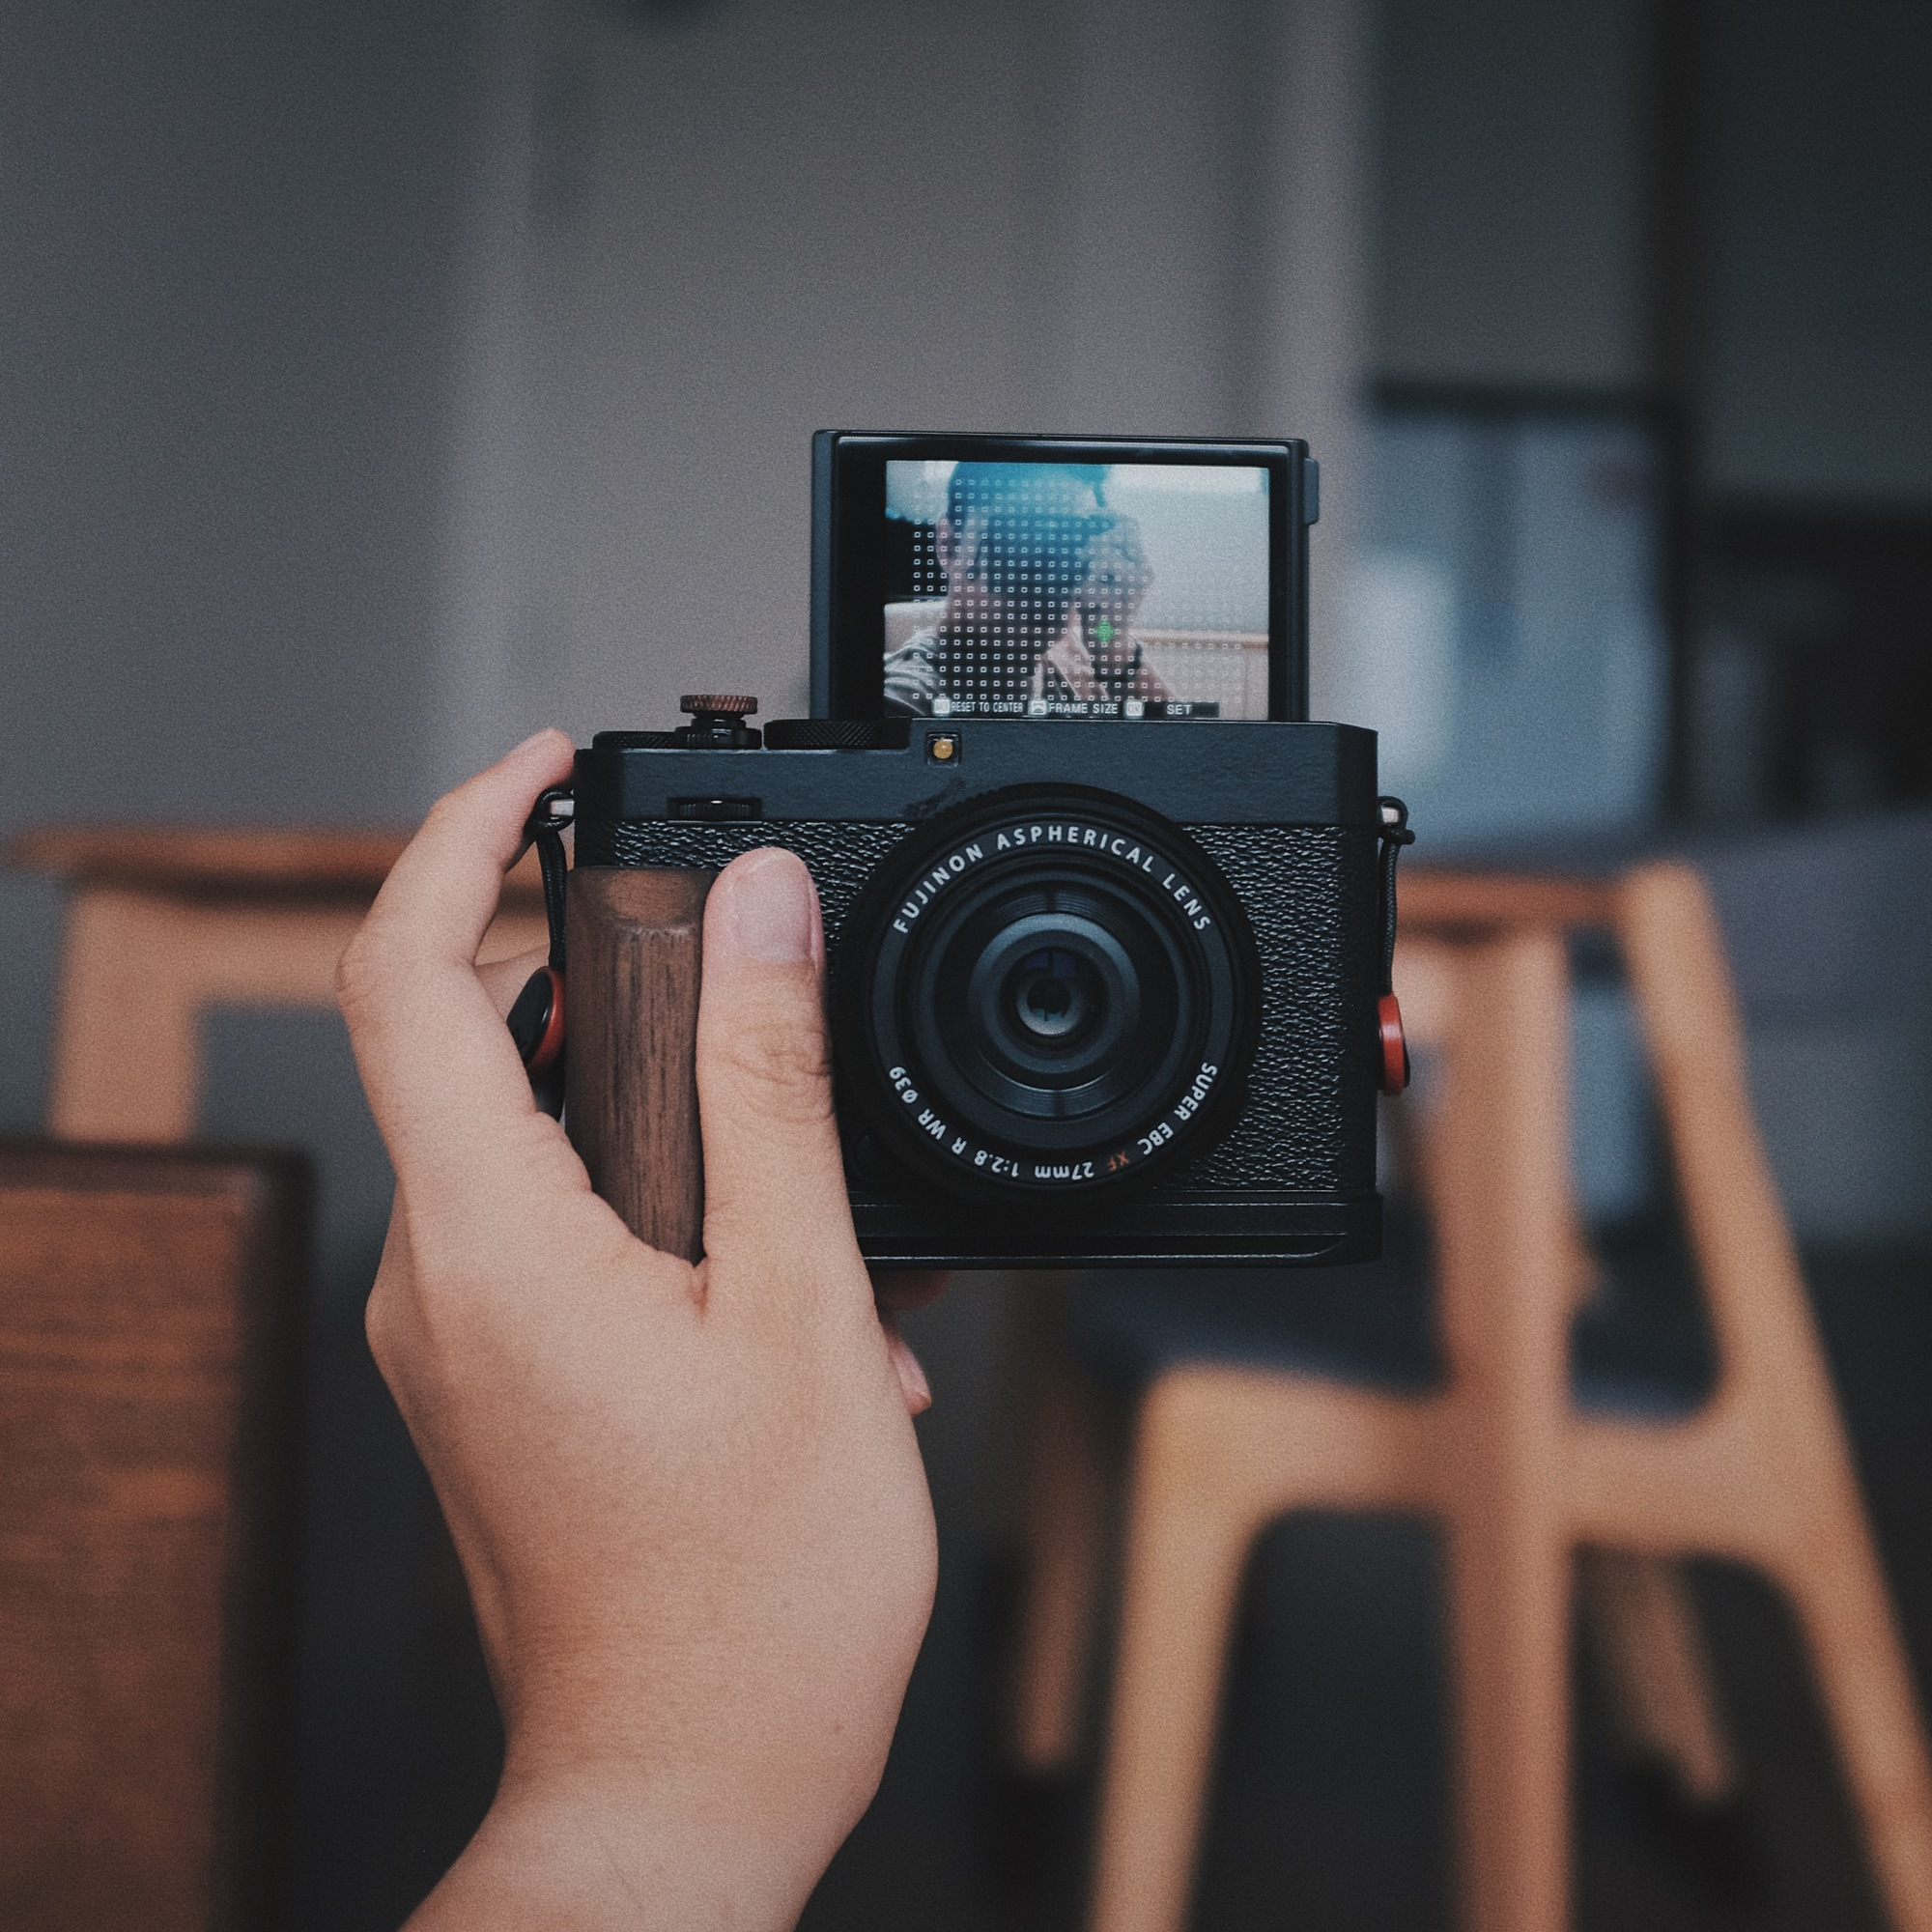
\includegraphics[width=\linewidth]{\envfinaldir/coverpic-prod.jpg}\par
            % \vskip 30pt
            \vfill

            \normalsize\rmfamily\scshape
            \copyright{} The Web Digest Project \hfill\large \envdatestr
        \end{center}
    \end{titlepage}
    % \restoregeometry
}
\newcommand{\simplehref}[1]{%
    \textcolor{blue!80!green}{\href{#1}{#1}}%
}
\renewcommand{\contentsname}{\center\Huge\sffamily\bfseries Contents\par\vskip 20pt}
\newcounter{ipartcounter}
\setcounter{ipartcounter}{0}
\newcommand{\ipart}[1]{
    % \vskip 20pt
    \clearpage
    \stepcounter{ipartcounter}
    \phantomsection
    \addcontentsline{toc}{chapter}{#1}
    % \begin{center}
    %     \Huge
    %     \sffamily\bfseries
    %     #1
    % \end{center}
    % \vskip 20pt plus 7pt
}
\newcounter{ichaptercounter}
\setcounter{ichaptercounter}{0}
\newcommand{\ichapter}[1]{
    % \vskip 20pt
    \clearpage
    \stepcounter{ichaptercounter}
    \phantomsection
    \addcontentsline{toc}{section}{\numberline{\arabic{ichaptercounter}}#1}
    \begin{center}
        \Huge
        \sffamily\bfseries
        #1
    \end{center}
    \vskip 20pt plus 7pt
}
\newcommand{\entrytitlefont}[1]{\subsection*{\raggedright\Large\sffamily\bfseries#1}}
\newcommand{\entryitemGeneric}[2]{
    % argv: title, url
    \parbox{\linewidth}{
        \entrytitlefont{#1}\par\vskip 5pt
        \footnotesize\ttfamily\mdseries
        \simplehref{#2}
    }\vskip 11pt plus 11pt minus 1pt
}
\newcommand{\entryitemGithub}[3]{
    % argv: title, url, desc
    \parbox{\linewidth}{
        \entrytitlefont{#1}\par\vskip 5pt
        \footnotesize\ttfamily\mdseries
        \simplehref{#2}\par\vskip 5pt
        \small\rmfamily\mdseries#3
    }\vskip 11pt plus 11pt minus 1pt
}
\newcommand{\entryitemAp}[3]{
    % argv: title, url, desc
    \parbox{\linewidth}{
        \entrytitlefont{#1}\par\vskip 5pt
        \footnotesize\ttfamily\mdseries
        \simplehref{#2}\par\vskip 5pt
        \small\rmfamily\mdseries#3
    }\vskip 11pt plus 11pt minus 1pt
}
\newcommand{\entryitemHackernews}[3]{
    % argv: title, hnurl, rawurl
    % \parbox{\linewidth}{
    %     \entrytitlefont{#1}\par\vskip 5pt
    %     \footnotesize\ttfamily\mdseries
    %     \simplehref{#3}\par
    %     \textcolor{black!50}{\href{#2}{#2}}
    % }\vskip 11pt plus 11pt minus 1pt
    \begin{minipage}{\linewidth}
            \entrytitlefont{#1}\par\vskip 5pt
            \footnotesize\ttfamily\mdseries
            \simplehref{#3}\par
            \textcolor{black!50}{\href{#2}{#2}}
    \end{minipage}\par\vskip 11pt plus 11pt minus 1pt
}







\begin{document}

\makeheader

\tableofcontents\clearpage




\ipart{Developers}
\ichapter{Hacker News}
\entryitemTwoLinks{Jeep owners fed up with in-car pop-up ads}{https://news.ycombinator.com/item?id=43272453}{https://www.kbb.com/car-news/jeep-owners-fed-up-with-in-car-pop-up-ads/}

\entryitemTwoLinks{Macron to open debate on extending French nuclear protection to European allies}{https://news.ycombinator.com/item?id=43271774}{https://www.reuters.com/world/europe/frances-macron-address-nation-late-wednesday-2025-03-05/}

\entryitemTwoLinks{NCSC, GCHQ, UK Gov't expunge advice to "use Apple encryption"}{https://news.ycombinator.com/item?id=43271177}{https://alecmuffett.com/article/112522}

\entryitemTwoLinks{QwQ-32B: Embracing the Power of Reinforcement Learning}{https://news.ycombinator.com/item?id=43270843}{https://qwenlm.github.io/blog/qwq-32b/}

\entryitemTwoLinks{Tailscale is pretty useful}{https://news.ycombinator.com/item?id=43270835}{https://blog.6nok.org/tailscale-is-pretty-useful/}

\entryitemTwoLinks{Skynet won and destroyed humanity}{https://news.ycombinator.com/item?id=43270687}{https://dmathieu.com/en/opinions/skynet-won/}

\entryitemTwoLinks{Apple takes UK to court over 'backdoor' order}{https://news.ycombinator.com/item?id=43270079}{https://www.theregister.com/2025/03/05/apple\_reportedly\_ipt\_complaint/}

\entryitemTwoLinks{There Was a Texas Lottery Arbitrage}{https://news.ycombinator.com/item?id=43269846}{https://www.bloomberg.com/opinion/articles/2025-03-05/there-was-a-texas-lottery-arbitrage}

\entryitemTwoLinks{My Beancount books are 95\% automatic after 3 years (2024)}{https://news.ycombinator.com/item?id=43268454}{https://fangpenlin.com/posts/2024/12/30/my-beancount-books-are-95-percent-automatic/}

\entryitemTwoLinks{Things we've learned about building products}{https://news.ycombinator.com/item?id=43267095}{https://newsletter.posthog.com/p/50-things-weve-learned-about-building}

\entryitemTwoLinks{MacBook Air M4}{https://news.ycombinator.com/item?id=43266537}{https://www.apple.com/macbook-air/}

\entryitemTwoLinks{Apple unveils new Mac Studio}{https://news.ycombinator.com/item?id=43266474}{https://www.apple.com/newsroom/2025/03/apple-unveils-new-mac-studio-the-most-powerful-mac-ever/}

\entryitemTwoLinks{Apple M3 Ultra}{https://news.ycombinator.com/item?id=43266453}{https://www.apple.com/newsroom/2025/03/apple-reveals-m3-ultra-taking-apple-silicon-to-a-new-extreme/}

\entryitemTwoLinks{Who's Afraid of Peter Thiel? A New Biography Suggests We All Should Be (2021)}{https://news.ycombinator.com/item?id=43265955}{https://time.com/6092844/peter-thiel-power-biography-the-contrarian/}

\entryitemTwoLinks{The Return of Digg, a Star of an Earlier Internet Era}{https://news.ycombinator.com/item?id=43265521}{https://www.nytimes.com/2025/03/05/technology/digg-alexis-ohanian-kevin-rose.html}

\entryitemTwoLinks{MS Paint IDE}{https://news.ycombinator.com/item?id=43265431}{https://ms-paint-i.de/}

\entryitemTwoLinks{NASA Successfully Acquires GPS Signals on Moon}{https://news.ycombinator.com/item?id=43265303}{https://www.nasa.gov/general/nasa-successfully-acquires-gps-signals-on-moon/}

\entryitemTwoLinks{'Shadow fleets' and sabotage: are Europe's undersea cables under attack?}{https://news.ycombinator.com/item?id=43265224}{https://www.theguardian.com/world/ng-interactive/2025/mar/05/shadow-fleets-subaquatic-sabotage-europe-undersea-internet-cables-under-attack}

\entryitemTwoLinks{Lynx: Open Source Native Cross Platform framework used in TikTok}{https://news.ycombinator.com/item?id=43264957}{https://lynxjs.org/blog/lynx-unlock-native-for-more.html}

\entryitemTwoLinks{Richard Sutton and Andrew Barto Win 2024 Turing Award}{https://news.ycombinator.com/item?id=43264847}{https://awards.acm.org/about/2024-turing}\ichapter{Phoronix}
\entryitemGeneric{\hskip 0pt{}Intel Engineers To Return To Working On Habana Labs Linux Driver, Gaudi 3 Expected}{https://www.phoronix.com/news/Intel-Habana-Labs-Upstream-2025}

\entryitemGeneric{\hskip 0pt{}Xen 4.20 Hypervisor Released With AMD Zen 5 Support, More Performance Optimizations}{https://www.phoronix.com/news/Xen-4.20-Released}

\entryitemGeneric{\hskip 0pt{}AMD Radeon RX 9070 + RX 9070 XT Linux Performance}{https://www.phoronix.com/review/amd-radeon-rx9070-linux}

\entryitemGeneric{\hskip 0pt{}AMD Radeon RX 9070 Series Linux GPU Compute Performance}{https://www.phoronix.com/review/amd-radeon-rx9070-linux-compute}

\entryitemGeneric{\hskip 0pt{}Making Vulkan More Of A "Joy To Use" Discussed At Vulkanised 2025}{https://www.phoronix.com/news/Vulkan-Joy-To-Use-2025}

\entryitemGeneric{\hskip 0pt{}FreeDesktop.org GitLab Will Be Down For Up To One Week Due To Cloud Migration}{https://www.phoronix.com/news/FreeDesktop-Down-1-Week-Soon}

\entryitemGeneric{\hskip 0pt{}Linux 6.15 Preparing Support For The XP-Pen Artist Pro 19, A Big 4K Drawing Tablet}{https://www.phoronix.com/news/Linux-6.15-XP-Pen-Artist-Pro-19}

\entryitemGeneric{\hskip 0pt{}More Apple SoC DeviceTree Additions Being Upstreamed For Linux 6.15}{https://www.phoronix.com/news/Apple-SoC-DT-Linux-6.15-2}

\entryitemGeneric{\hskip 0pt{}AMD ZenDNN 5.0.1 Released To Help With EPYC Inferencing For Recommender Systems \& LLMs}{https://www.phoronix.com/news/AMD-ZenDNN-5.0.1}\ichapter{Dribbble}
\entryitemGeneric{\hskip 0pt{}Puzzle Fintech Website Design}{https://dribbble.com/shots/25651990-Puzzle-Fintech-Website-Design}

\entryitemGeneric{\hskip 0pt{}Real Estate Platform UI}{https://dribbble.com/shots/25711538-Real-Estate-Platform-UI}

\entryitemGeneric{\hskip 0pt{}Logistics Company Web Design Landing Page}{https://dribbble.com/shots/25708252-Logistics-Company-Web-Design-Landing-Page}

\entryitemGeneric{\hskip 0pt{}Letter C + Hummingbird}{https://dribbble.com/shots/25713900-Letter-C-Hummingbird}

\entryitemGeneric{\hskip 0pt{}Inner Truth}{https://dribbble.com/shots/25659901-Inner-Truth}

\entryitemGeneric{\hskip 0pt{}Easy A Deck}{https://dribbble.com/shots/25715917-Easy-A-Deck}

\entryitemGeneric{\hskip 0pt{}Star + Check Mark Icon Concept}{https://dribbble.com/shots/25709690-Star-Check-Mark-Icon-Concept}

\entryitemGeneric{\hskip 0pt{}FREELANCE (Finally)}{https://dribbble.com/shots/25710537-FREELANCE-Finally}

\entryitemGeneric{\hskip 0pt{}Recent Logo Designs - Jeroen van Eerden}{https://dribbble.com/shots/25709914-Recent-Logo-Designs-Jeroen-van-Eerden}

\entryitemGeneric{\hskip 0pt{}Wolf}{https://dribbble.com/shots/25707625-Wolf}

\entryitemGeneric{\hskip 0pt{}Star + Check Mark Icon Concept}{https://dribbble.com/shots/25698016-Star-Check-Mark-Icon-Concept}

\entryitemGeneric{\hskip 0pt{}Block13 Promo Board Design /1 /2 /3}{https://dribbble.com/shots/25700177-Block13-Promo-Board-Design-1-2-3}

\entryitemGeneric{\hskip 0pt{}Communication Illustration}{https://dribbble.com/shots/25700541-Communication-Illustration}

\entryitemGeneric{\hskip 0pt{}Tally Logo Design}{https://dribbble.com/shots/25693309-Tally-Logo-Design}

\entryitemGeneric{\hskip 0pt{}Letter A}{https://dribbble.com/shots/25691267-Letter-A}

\entryitemGeneric{\hskip 0pt{}Detective Dog Logo}{https://dribbble.com/shots/25692587-Detective-Dog-Logo}

\entryitemGeneric{\hskip 0pt{}HyperSeed - Logo Design}{https://dribbble.com/shots/25692269-HyperSeed-Logo-Design}

\entryitemGeneric{\hskip 0pt{}Logo Design for Gaming Platform (Unused for Sale)}{https://dribbble.com/shots/25692257-Logo-Design-for-Gaming-Platform-Unused-for-Sale}

\entryitemGeneric{\hskip 0pt{}NonStop}{https://dribbble.com/shots/25692105-NonStop}

\entryitemGeneric{\hskip 0pt{}Barbershop app dashboard}{https://dribbble.com/shots/25687859-Barbershop-app-dashboard}

\entryitemGeneric{\hskip 0pt{}Jiggy's Court™}{https://dribbble.com/shots/25693857-Jiggy-s-Court}

\entryitemGeneric{\hskip 0pt{}Finance app ui Design}{https://dribbble.com/shots/25691020-Finance-app-ui-Design}

\entryitemGeneric{\hskip 0pt{}—From Archive (Pt. 10)}{https://dribbble.com/shots/25692986--From-Archive-Pt-10}

\entryitemGeneric{\hskip 0pt{}Block13 Promo Board Design 2}{https://dribbble.com/shots/25694586-Block13-Promo-Board-Design-2}


\ipart{Developers~~~~(zh-Hans)}
\ichapter{Solidot}
\entryitemGeneric{\hskip 0pt{}2024 年图灵奖授予了奠定强化学习的计算机科学家 Andrew Barto 和 Richard Sutton}{https://www.solidot.org/story?sid=80720}

\entryitemGeneric{\hskip 0pt{}苹果对英国的后门命令提起上诉}{https://www.solidot.org/story?sid=80719}

\entryitemGeneric{\hskip 0pt{}科学家创造猛犸鼠}{https://www.solidot.org/story?sid=80718}

\entryitemGeneric{\hskip 0pt{}TCL 在高端电视机出货量上超过 LG 仅次于三星}{https://www.solidot.org/story?sid=80717}

\entryitemGeneric{\hskip 0pt{}宇宙最早的水可能形成于大爆炸后的 1-2 亿年}{https://www.solidot.org/story?sid=80716}

\entryitemGeneric{\hskip 0pt{}韦伯望远镜发现有复杂大气层的流浪行星}{https://www.solidot.org/story?sid=80715}

\entryitemGeneric{\hskip 0pt{}兄弟打印机通过强制性更新固件禁用第三方墨盒}{https://www.solidot.org/story?sid=80714}

\entryitemGeneric{\hskip 0pt{}Homebrew Computer Club 成立 50 周年}{https://www.solidot.org/story?sid=80713}

\entryitemGeneric{\hskip 0pt{}Firefox 136 释出,支持垂直标签}{https://www.solidot.org/story?sid=80712}

\entryitemGeneric{\hskip 0pt{}阿斯巴甜会导致动物体内胰岛素水平上升}{https://www.solidot.org/story?sid=80710}

\entryitemGeneric{\hskip 0pt{}台积电计划向美国追加投资千亿美元}{https://www.solidot.org/story?sid=80709}

\entryitemGeneric{\hskip 0pt{}报告称中国的芯片论文数及高引用论文数超越美国}{https://www.solidot.org/story?sid=80708}

\entryitemGeneric{\hskip 0pt{}大脑微塑料水平与痴呆症相关}{https://www.solidot.org/story?sid=80707}

\entryitemGeneric{\hskip 0pt{}AI 娱乐公司以模因币竞标 Infowars}{https://www.solidot.org/story?sid=80706}

\entryitemGeneric{\hskip 0pt{}火星的红色可能来自水铁矿}{https://www.solidot.org/story?sid=80705}

\entryitemGeneric{\hskip 0pt{}拯救了 240 万婴儿的澳大利亚人 James Harrison 去世}{https://www.solidot.org/story?sid=80704}

\entryitemGeneric{\hskip 0pt{}欧洲刑警组织逮捕 25 名分享 AI 儿童色情的用户}{https://www.solidot.org/story?sid=80703}

\entryitemGeneric{\hskip 0pt{}芹菜西兰花中的天然成分能抑制白发}{https://www.solidot.org/story?sid=80702}

\entryitemGeneric{\hskip 0pt{}美国将设加密货币战略储备}{https://www.solidot.org/story?sid=80701}

\entryitemGeneric{\hskip 0pt{}新方头鱼物种以《幽灵公主》角色命名}{https://www.solidot.org/story?sid=80700}\ichapter{V2EX}
\entryitemGeneric{\hskip 0pt{}[分享发现] 克隆网站}{https://www.v2ex.com/t/1116218}

\entryitemGeneric{\hskip 0pt{}[分享创造] [开源]🚀 Certimate v0.3.0 正式发布:更强大、更灵活的 SSL 证书管理!}{https://www.v2ex.com/t/1116217}

\entryitemGeneric{\hskip 0pt{}[分享创造] 在 V2EX 发帖 12 个小时, Chrome 插件获得用户查看/安装数量统计}{https://www.v2ex.com/t/1116216}

\entryitemGeneric{\hskip 0pt{}[阅读] 2025 二月读地球科学 设计理论 文学小说 传记 佛经…… 10 本}{https://www.v2ex.com/t/1116215}

\entryitemGeneric{\hskip 0pt{}[Apple] 选择困难,求治。}{https://www.v2ex.com/t/1116214}

\entryitemGeneric{\hskip 0pt{}[分享发现] Manus.AI 深夜发布...Discord 半夜挤满了求内测码的人}{https://www.v2ex.com/t/1116213}

\entryitemGeneric{\hskip 0pt{}[职场话题] 绩效 B,是不是扯淡}{https://www.v2ex.com/t/1116212}

\entryitemGeneric{\hskip 0pt{}[程序员] 对于 cursor 最近的一些感悟}{https://www.v2ex.com/t/1116211}

\entryitemGeneric{\hskip 0pt{}[问与答] 你身边有没有总是喜欢找你借钱的人?}{https://www.v2ex.com/t/1116210}

\entryitemGeneric{\hskip 0pt{}[分享发现] 什么年代了, mstsc 远程桌面与 ssh 的文件传输速度问题,仍然没改进}{https://www.v2ex.com/t/1116209}

\entryitemGeneric{\hskip 0pt{}[macOS] 新款 M4 MacBook Air 可以外接俩个显示器了}{https://www.v2ex.com/t/1116208}

\entryitemGeneric{\hskip 0pt{}[程序员] 现在的 AI 的缺乏直觉和经验,这一点相对人类还是无可替代,从一个例子说明}{https://www.v2ex.com/t/1116207}

\entryitemGeneric{\hskip 0pt{}[分享创造] [开源] Dock Video Player}{https://www.v2ex.com/t/1116206}

\entryitemGeneric{\hskip 0pt{}[酷工作] 北京五道口 AI 创业公司,前景好,招 AI 工程师/nodejs/rn/数据分析/市场/产品运营等}{https://www.v2ex.com/t/1116205}

\entryitemGeneric{\hskip 0pt{}[求职] 郑州:8 年全栈开发求职,golang,vue}{https://www.v2ex.com/t/1116204}

\entryitemGeneric{\hskip 0pt{}[硬件] x99 主板鸡血后, cpu 温度 73 度,是因为散热器是 9cm 的吗?}{https://www.v2ex.com/t/1116202}

\entryitemGeneric{\hskip 0pt{}[Mac Studio] M3 Ultra 的 Mac studio 或许是本地部署大模型的最佳利器?}{https://www.v2ex.com/t/1116201}

\entryitemGeneric{\hskip 0pt{}[分享创造] [旅行 APP 产品诞生日记] 7day/100days}{https://www.v2ex.com/t/1116200}

\entryitemGeneric{\hskip 0pt{}[求职] 深圳有没有招女程序员的?写 Python 的。}{https://www.v2ex.com/t/1116199}

\entryitemGeneric{\hskip 0pt{}[问与答] 批量音频 MP3 文件转文本,哪个软件识别率最好}{https://www.v2ex.com/t/1116198}

\entryitemGeneric{\hskip 0pt{}[PHP] 想用 PHP 做微服务开发,有偿求指导}{https://www.v2ex.com/t/1116197}

\entryitemGeneric{\hskip 0pt{}[Apple] M3 Ultra + 512GB 能跑 671B 全量 Deepseek R1 了么?}{https://www.v2ex.com/t/1116196}

\entryitemGeneric{\hskip 0pt{}[问与答] 请问有没有开源的客服系统啊}{https://www.v2ex.com/t/1116195}

\entryitemGeneric{\hskip 0pt{}[macOS] 如何在 x86 的 macOS 上运行 arm64 的 macOS}{https://www.v2ex.com/t/1116194}

\entryitemGeneric{\hskip 0pt{}[MacBook Air] 新的 M4 macbook Air 发售了!有新颜色 天蓝色!}{https://www.v2ex.com/t/1116193}

\entryitemGeneric{\hskip 0pt{}[分享发现] 2024 TED 精选分享}{https://www.v2ex.com/t/1116192}

\entryitemGeneric{\hskip 0pt{}[酷工作] 远程岗位-量化做市团队招聘 开发工程师(golang,c++, 高频)}{https://www.v2ex.com/t/1116191}

\entryitemGeneric{\hskip 0pt{}[iPad] iPad mini 最新系统 iPad OS18 不自动填充各个软件的密码?}{https://www.v2ex.com/t/1116189}

\entryitemGeneric{\hskip 0pt{}[Linux] 大佬们求助,硬盘没法格式化/dev/sda1 is apparently in use by the system; will not make a filesystem here!}{https://www.v2ex.com/t/1116187}

\entryitemGeneric{\hskip 0pt{}[微信] xposed 企业微信打卡虚拟定位问题}{https://www.v2ex.com/t/1116185}

\entryitemGeneric{\hskip 0pt{}[Apple] 苹果刚刚推出了新款 Mac Studio}{https://www.v2ex.com/t/1116184}

\entryitemGeneric{\hskip 0pt{}[Local LLM] Intel GPU 的 llama-bench 测试结果}{https://www.v2ex.com/t/1116183}

\entryitemGeneric{\hskip 0pt{}[Apple] MacBook Air 已更新 M4, Mac Studio 已更新 M4 Max 或 M3 Ultra}{https://www.v2ex.com/t/1116182}

\entryitemGeneric{\hskip 0pt{}[Firefox] Firefox 最新版(v136.0)更新原生支持垂直标签页了!}{https://www.v2ex.com/t/1116181}

\entryitemGeneric{\hskip 0pt{}[分享发现] 推上向 grok 问的问题和''为你推荐''信息流原来是联动的}{https://www.v2ex.com/t/1116180}

\entryitemGeneric{\hskip 0pt{}[生活] 人类的命运无常,悲欢不同}{https://www.v2ex.com/t/1116179}

\entryitemGeneric{\hskip 0pt{}[问与答] 如何在 Windows 终端下打开 Obsidian? call start /d 命令无法正常打开。}{https://www.v2ex.com/t/1116177}

\entryitemGeneric{\hskip 0pt{}[求职] 杭州终端安全业务相关的安全仔有人要吗}{https://www.v2ex.com/t/1116176}

\entryitemGeneric{\hskip 0pt{}[问与答] 做文字游戏遇到摆烂同行怎么办}{https://www.v2ex.com/t/1116175}

\entryitemGeneric{\hskip 0pt{}[DNS] 自建 DNS 相关分享}{https://www.v2ex.com/t/1116172}

\entryitemGeneric{\hskip 0pt{}[分享发现] 坚果云 Mac 史诗级更新}{https://www.v2ex.com/t/1116171}

\entryitemGeneric{\hskip 0pt{}[Google] google cloud function 需要每 3 分钟调用一次}{https://www.v2ex.com/t/1116170}

\entryitemGeneric{\hskip 0pt{}[问与答] 华为不是算车子的解决方案供应商嘛?为什么会让供应商开发布会啊?}{https://www.v2ex.com/t/1116169}

\entryitemGeneric{\hskip 0pt{}[问与答] clash meta for android 如何自动应用 Shadowrocket-ADBlock-Rules-Forever ?}{https://www.v2ex.com/t/1116167}

\entryitemGeneric{\hskip 0pt{}[OpenWrt] 分享我的一个 openclash 终极优化方案}{https://www.v2ex.com/t/1116166}

\entryitemGeneric{\hskip 0pt{}[程序员] 请教后端面试官们, 现在面试还会对候选人深究八股文吗}{https://www.v2ex.com/t/1116165}

\entryitemGeneric{\hskip 0pt{}[问与答] 从哪里开始着手学 AI 大模型呢?导师给了张下面这个图,然后自学。但没有头绪}{https://www.v2ex.com/t/1116164}

\entryitemGeneric{\hskip 0pt{}[iPad] Apple 官网调整国行 iPad mini(A17 Pro)售价}{https://www.v2ex.com/t/1116163}

\entryitemGeneric{\hskip 0pt{}[问与答] 在线给狗子征集一个英文名,母的白色柴犬 名字叫蛋黄}{https://www.v2ex.com/t/1116162}

\entryitemGeneric{\hskip 0pt{}[问与答] ⚫``模拟按住浏览器滚动条怎样实现?''⚫}{https://www.v2ex.com/t/1116161}


\ipart{Generic News}







\clearpage
\leavevmode\vfill
\footnotesize

Copyright \copyright{} 2023-2025 Neruthes and other contributors.

This document is published with CC BY-NC-ND 4.0 license.

The entries listed in this newsletter may be copyrighted by their respective creators.

This newsletter is generated by the Web Digest project.

The newsletters are also delivered via Telegram channel \CJKunderline{\href{https://t.me/webdigestchannel}{https://t.me/webdigestchannel}}.\\
RSS feed is available at \CJKunderline{\href{https://webdigest.pages.dev/rss.xml}{https://webdigest.pages.dev/rss.xml}}.

This newsletter is available in PDF at
\CJKunderline{\href{https://webdigest.pages.dev/}{https://webdigest.pages.dev/}}.

The source code being used to generate this newsletter is available at\\
\CJKunderline{\href{https://github.com/neruthes/webdigest}{https://github.com/neruthes/webdigest}}.

This newsletter is also available in
\CJKunderline{\href{http://webdigest.pages.dev/readhtml/\envyear/WebDigest-20250306.html}{HTML}} and
\CJKunderline{\href{https://github.com/neruthes/webdigest/blob/master/markdown/\envyear/WebDigest-20250306.md}{Markdown}}.


\coverpic{https://unsplash.com/photos/a-pink-and-yellow-background-with-a-round-object-in-the-middle-V8GVT2XQ5oc}{Andrei J Castanha}


\end{document}
